\documentclass{article}
\usepackage[utf8]{inputenc}
\usepackage{hyperref}
\usepackage[letterpaper, portrait, margin=1in]{geometry}
\usepackage{enumitem}
\usepackage{amsmath}
\usepackage{booktabs}
\usepackage{graphicx}

\usepackage{hyperref}
\hypersetup{
colorlinks=true,
    linkcolor=black,
    filecolor=black,      
    urlcolor=blue,
    citecolor=black,
}
\usepackage{natbib}

\usepackage{titlesec}
  
\title{ECON 7103 Homework 2}
\author{Ioanna Maria Spyrou}
\date{Spring semester 2021}
  
\begin{document}
  
\maketitle


\section{Question 1}

\begin{table}[h]
    \centering
    \begin{tabular}{llll}
\toprule
{} & control mean & treated mean & p-values \\
{} &       (s.d.) & \multicolumn{2}{l}{(s.d)} \\
\midrule
electricity &      1181.33 &      1086.75 &   (0.00) \\
            &     (454.31) &     (423.96) &          \\
sqft        &      1633.05 &      1657.55 &   (0.57) \\
            &     (682.90) &     (686.27) &          \\
temp        &        79.89 &        79.89 &   (0.99) \\
            &       (2.16) &       (1.97) &          \\
\bottomrule
\end{tabular}

    \caption{Mean table.}
    \label{tab:my_label}
\end{table}

According to Table 1 the difference in mean of electricity use between the two groups is statistically significant since the p-value is 0. For the other two variables the difference in means is not significant based on the p-values. So randomization worked.

\section{Question 2}
Figure 1 depicts Kernel density plot of electricity use for the two groups.

\begin{figure}[ht]
    \centering
    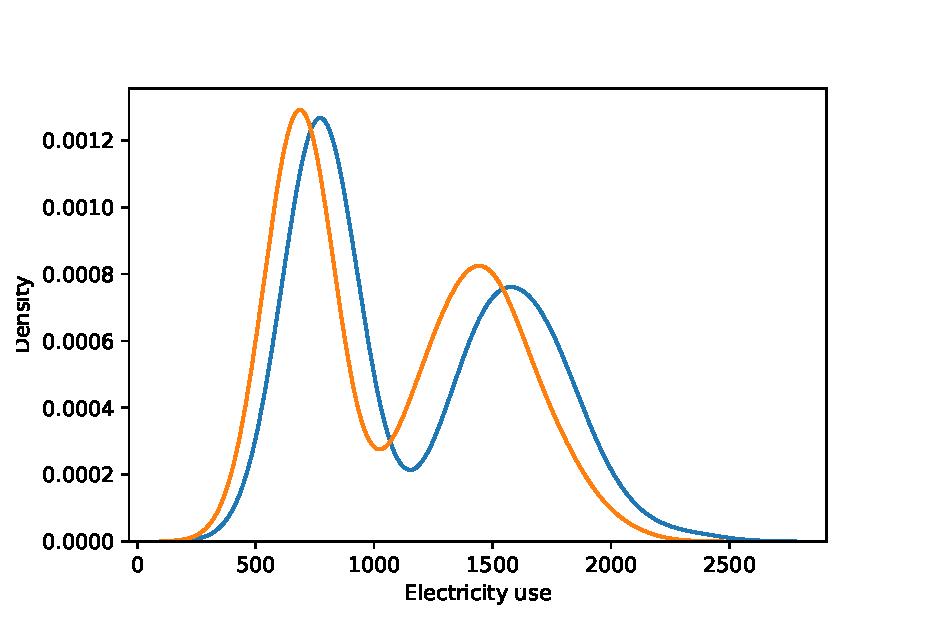
\includegraphics[scale = 0.7]{plot.eps}
    \caption{Sample kernel density plot of electricity use.}
    \label{fig:plot}
\end{figure}

The retrofit program reduces the consumption of electricity, since the electricity consumption in the treated group is less compared to control group.

\section{Question 3}
The values for $\beta$ array using the three approaches are similar and are given below:\\
\\a)
$$\beta_0 = -83.60275758$$
$$\beta_{sqft} = 0.61533854$$
$$\beta_{retrofit} =-109.66617626$$
$$\beta_{temp} = 3.25507541$$\\
\\b)
$$\beta_0 = -83.472798910$$
$$\beta_{sqft} = 0.6153380940$$
$$\beta_{retrofit} =-109.666428586$$
$$\beta_{temp} = 3.25346038$$\\
\\c)
$$\beta_0 = -83.6028$$
$$\beta_{sqft} = 0.6153$$
$$\beta_{retrofit} =-109.6662$$
$$\beta_{temp} = 3.2551$$
\end{document}